\documentclass[tikz,border=5pt]{standalone}
\usepackage{pgfplots}
\pgfplotsset{compat=1.18}

\definecolor{corba}{HTML}{365FB3}
\definecolor{punt}{HTML}{B91C1C}
\definecolor{guia}{HTML}{6B7280}

\begin{document}
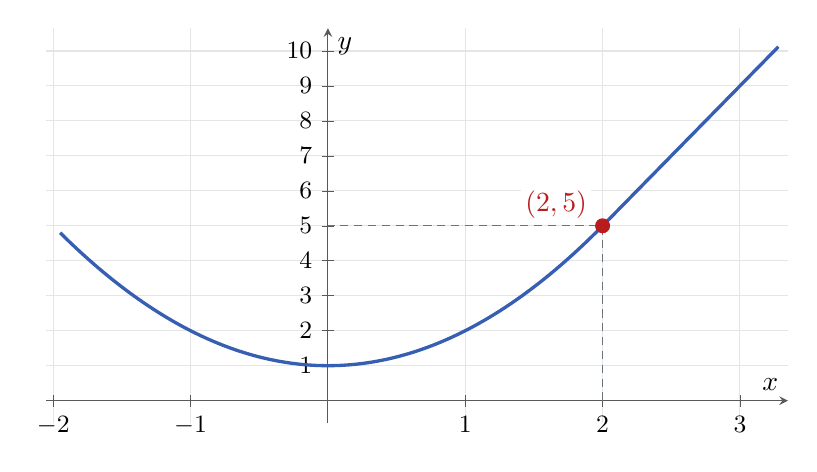
\begin{tikzpicture}
  \begin{axis}[
    width=11cm,
    height=6.6cm,
    axis lines=middle,
    xmin=-2.05,
    xmax=3.35,
    ymin=-0.65,
    ymax=10.65,
    xlabel={$x$},
    ylabel={$y$},
    xtick={-2,-1,0,1,2,3},
    ytick={1,2,3,4,5,6,7,8,9,10},
    grid=major,
    grid style={black!10},
    axis line style={black!65},
    tick style={black!65},
    tick label style={font=\small},
    clip=false,
  ]
    \addplot[corba, very thick, domain=-1.95:2, samples=150] {x^2+1};
    \addplot[corba, very thick, domain=2:3.28, samples=80] {4*x-3};
    \draw[guia, densely dashed]
      (axis cs:2,0) -- (axis cs:2,5) -- (axis cs:0,5);
    \addplot[only marks, mark=*, mark size=2.5pt, punt]
      coordinates {(2,5)};
    \node[anchor=south east, text=punt, fill=white, inner sep=1.5pt]
      at (axis cs:1.92,5.08) {$(2,5)$};
  \end{axis}
\end{tikzpicture}
\end{document}
